次に,$X_{i}$の数が変化したときにステップ間の平均移動距離$\phi$がどう変化するかについて見てみることにする。このとき,点$x$の総数$M$と$X_{i}$の数$N$,$X_{i}$あたりの点の数$S$の間には比例の関係($M=N\times S$)が成り立っており,$N$を増やすことと$S$を増やすことはこの場合等価であるから,より細かく値を刻むことのできる$S$を変化させたときのクラスター数との間の関係について調べた。横軸を$S$,縦軸を平均のステップ間距離$\phi$としたグラフを図\ref{fig:f19}に示す。このときの$N$は$N=6$であり,$r=0.07$で,100回の試行を平均したものとなっている。
\begin{figure}[H]
    \begin{center}
        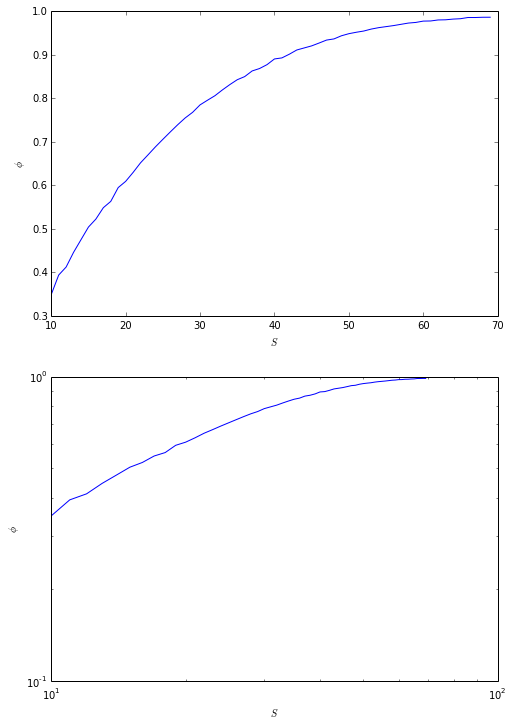
\includegraphics[width=10cm]{../img/S_phi_1.png}
        \caption{$S$を変化させたときのステップ間の平均距離}
        \label{fig:f19}
    \end{center}
\end{figure}

\subsection{解析的な計算}
以下に示すのは,これまで調べてきた性質が,解析的な計算によって求められないかと考えて行った試行である。

まず,点の分布する範囲は$\Omega = [0,1]\times [0,1]$であり,この中の面積$S$の領域の中に点を見出す確率は$S$である。

次に,領域内のある点$\vec x=(x,y)$を中心として半径$r$($0 < r \le 0.5$)の領域$B(\vec x, r)$内に点を見出す確率$p(\vec x)$は,境界の影響をうけない領域($\Omega ' = \{(x,y) | r \le x \le 1-r, r \le y \le 1-r \}$)では$\pi r^{2}$であり,境界の影響を受ける領域($\Omega'' = \Omega / \Omega'$)において点を見出す確率は,領域を
\begin{align}
\Omega''_{x} &= \{(x,y) | 0 \le x < r, r< y < 1-r\}\nonumber \\
\Omega''_{1-x} &= \{(x,y) | 1-r < x \le 1, r< y < 1-r\}\nonumber \\
\Omega''_{y} &= \{(x,y) | r < x < 1-r, 0 \le y < r\}\nonumber \\
\Omega''_{1-y} &= \{(x,y) | r < x < 1-r, 1-r < y \le 1\}\nonumber \\
\Omega''_{x,y} &= \{(x,y) | 0 \le x < r, 0 \le y < r\}\nonumber \\
\Omega''_{1-x,y} &= \{(x,y) | 1-r < x \le 1, 0 \le y < r\}\nonumber \\
\Omega''_{x,1-y} &= \{(x,y) | 0 \le x < r, 1-r < y \le 1\}\nonumber \\
\Omega''_{1-x, 1-y} &= \{(x,y) | 1-r < x \le 1, 1-r < y \le 1\}\nonumber
\end{align}
のようにあらわして,それぞれ考えることにする(図\ref{fig:f20})。
\begin{figure}[H]
    \begin{center}
        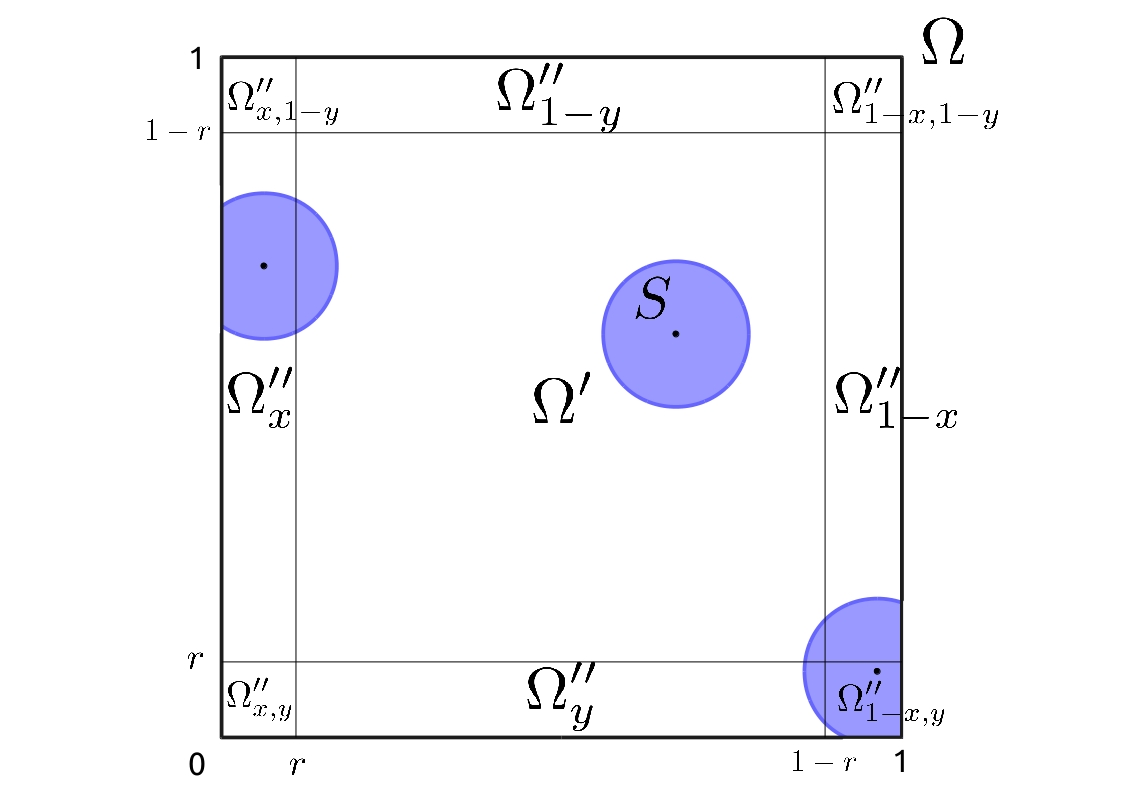
\includegraphics[width=10cm]{../img/omega.jpg}
        \caption{領域$\Omega$を分割した各領域}
        \label{fig:f20}
    \end{center}
\end{figure}
$\Omega''_{i} = \{\Omega''_{x}, \Omega''_{1-x}, \Omega''_{y}, \Omega''_{1-y}$\},また$\Omega''_{i,j} = \{\Omega''_{x,y}, \Omega''_{1-x,y}, \Omega''_{x,1-y}, \Omega''_{1-x,1-y}\}$でまとめて書くことにすると,
\[p(r)_{\Omega''_{i}} = i \sqrt{r^{2}-i^{2}} + r^{2} \left[ \pi -\arccos \frac{i}{r} \right]\]
\begin{figure}[H]
    \begin{center}
        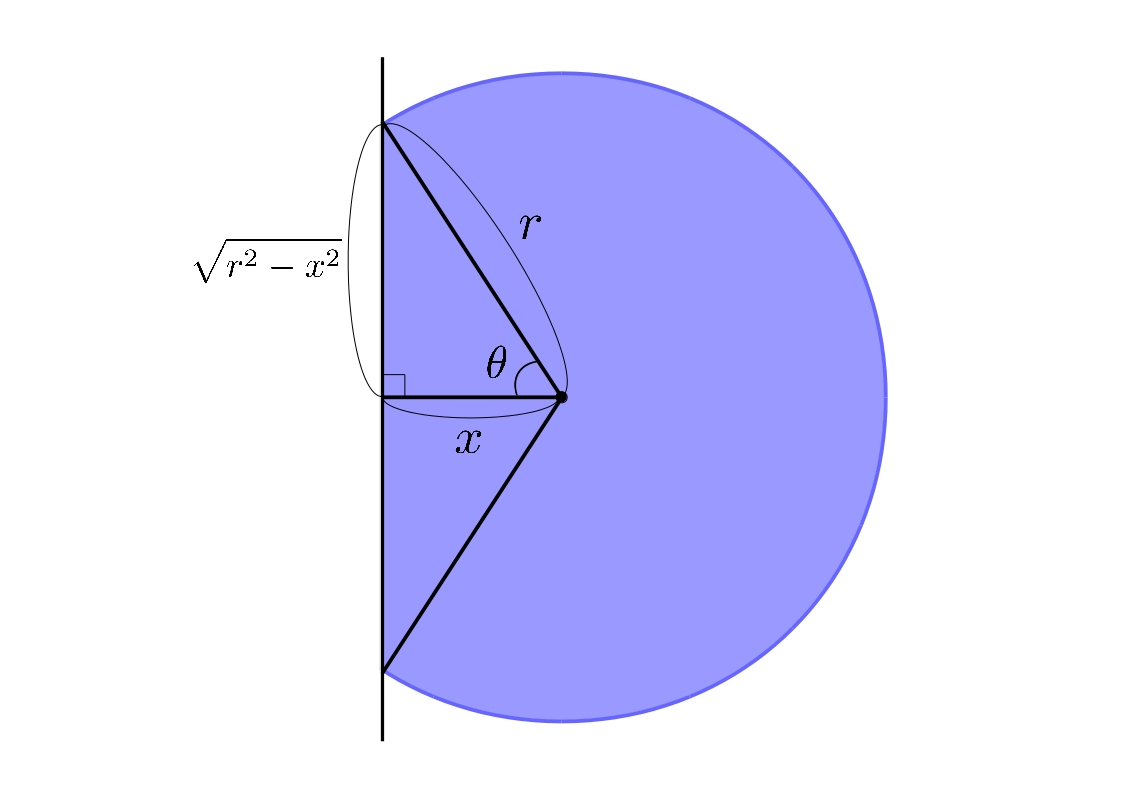
\includegraphics[width=10cm]{../img/omega_x.jpg}
        \caption{$\vec{x} \in \Omega''_{x}$であるときの面積$S$の求め方}
        \label{fig:f21}
    \end{center}
\end{figure}
\begin{align}p(r)_{\Omega''_{i,j}} = &\frac{1}{2}\left\{ \sqrt{r^{2}-i^{2}} + \min \left(j, \sqrt{r^{2}-i^{2}}\right) \right\}i + \frac{1}{2}\left\{ \sqrt{r^{2}-j^{2}} + \min \left( i, \sqrt{r^{2}-j^{2}}\right) \right\}j \nonumber \\
&+ \frac{1}{2}r^{2} \left\{ 2\pi -\arccos \frac{i}{r}-\arccos \frac{j}{r}-\min \left( \frac{\pi}{2}, \arccos \frac{i}{r} +\arccos \frac{j}{r} \right) \right\}
\end{align}
のようにあらわすことができる。
\begin{figure}[H]
    \begin{center}
        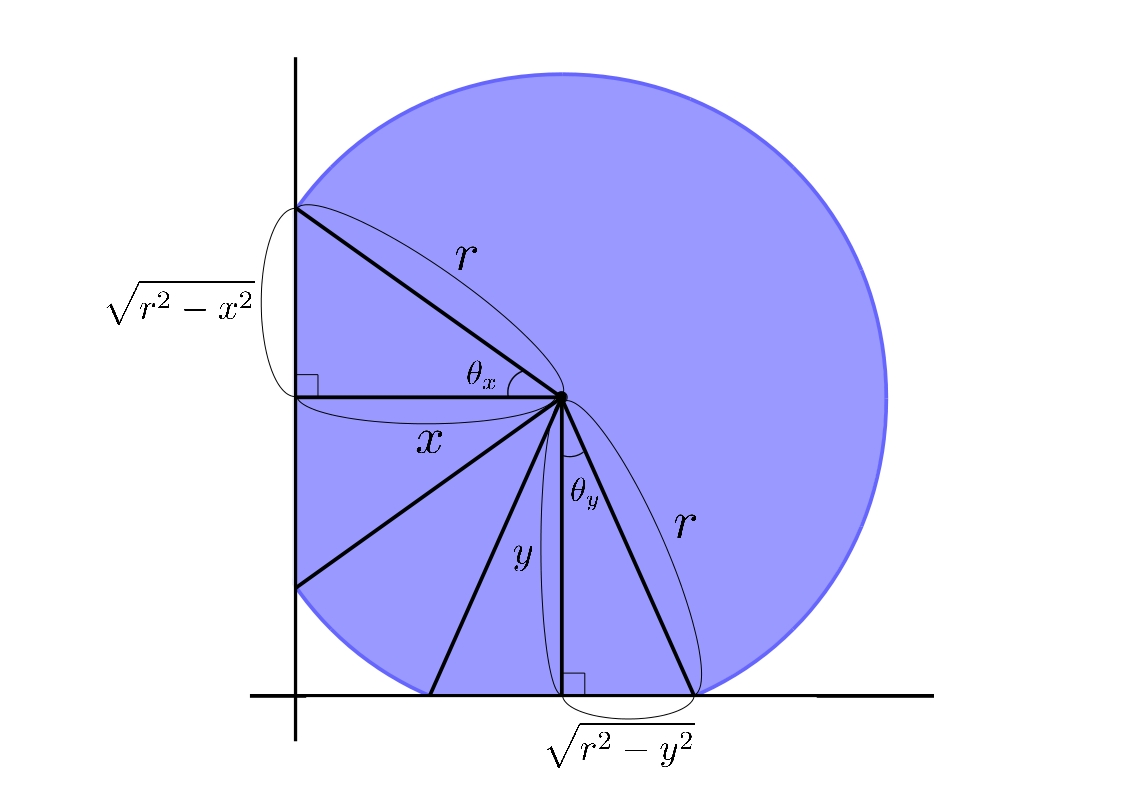
\includegraphics[width=10cm]{../img/omega_xy.jpg}
        \caption{$\vec{x} \in \Omega''_{x,y}$のときの面積$S$の求め方の一例}
        \label{fig:f22}
    \end{center}
\end{figure}

確率$p$をすべての領域について積分した値は,領域$\Omega$から一様乱数によって一つの点を選び,その点を中心とした$r$による範囲に1つの点を見出す確率の期待値となる。
この確率を$p'(r)$とし,$0\le r \le 0.5$のときは
\[p'(r) = p'(r)_{\Omega''} + 4p'(r)_{\Omega''_{i}} + 4p'(r)_{\Omega''_{i,j}}\]
とできる。それぞれの領域について積分を実行する。
\[p'(r)_{\Omega'} = \int_{r}^{1-r} \int_{r}^{1-r}\pi r^{2}\mathrm{d}x\mathrm{d}y = (1-2r)^{2}\pi r^{2}\]
\begin{align}
p'(r)_{\Omega'_{i}} = p'(r)_{\Omega'_{x}} &= \int_{0}^{r} \int_{r}^{1-r}\mathrm{d}x\mathrm{d}y\ x\sqrt{r^{2}-x^{2}} + r^{2}\left[\pi - \arccos\frac{x}{r}\right]\nonumber \\
&= (1-2r)\left\{ \frac{r^{3}}{3} + r^{2}\pi\cdot r - r^{2}\cdot r \right\}\nonumber \\
&= (1-2r)r^{3}\left( \pi-\frac{2}{3} \right)
\end{align}

NOTE1:
\begin{align}
&\int_{0}^{r}\mathrm{d}x\ x\sqrt{r^{2}-x^{2}} \nonumber \\
&\ \ \ \ \ \left[x = r\cos \theta \right]\nonumber \\
&= \int_{\frac{\pi}{2}}^{0}\mathrm{d}\theta\ (-r\sin\theta)\ r\cos\theta\ r\sin\theta\nonumber \\
&= r^{3}\left[ \frac{\sin^{3}\theta}{3}\right]^{\frac{\pi}{2}}_{0} \nonumber \\
&= \frac{r^{3}}{3}
\end{align}

NOTE2:
$x = \cos t \ (0< t< \pi)$とすると
\[\frac{\mathrm{d}x}{\mathrm{d}t} = - \sin t < 0\]
$t = \arccos x$であるから,
\begin{align}
\frac{\mathrm{d}}{\mathrm{d}x}\arccos x &= \frac{1}{\frac{\mathrm{d}}{\mathrm{d}t}\cos t} = -\frac{1}{\sin t}\nonumber \\
&=- \frac{1}{\sqrt{\sin^{2}t}} = - \frac{1}{\sqrt{1- \cos^{2}t}} \nonumber \\
&= - \frac{1}{\sqrt{1- x^{2}}}
\end{align}
したがって,
\begin{align}
\int \arccos x \mathrm{d}x\  &= x\arccos x + \int \frac{x}{\sqrt{1-x^{2}}}\mathrm{d}x\nonumber \\
&=x\arccos x - \sqrt{1-x^{2}} + C
\end{align}
($C$は積分定数)

今の場合,
\begin{align}
\int^{r}_{0} \arccos \frac{x}{r} \mathrm{d}x &= \int^{1}_{0}\arccos t \cdot r\mathrm{d}t\nonumber \\
&= r \left[ t \arccos t - \sqrt{1-t^{2}} \right]^{1}_{0}\nonumber \\
&= r ( 1\arccos1 -\sqrt{1-1} - 0 \arccos0 + \sqrt{1-0})\nonumber \\
&= r
\end{align}

$p'(r)_{\Omega''_{i,j}}$を以下のように分解してそれぞれ計算する。
\begin{align}
p'(r)_{\Omega''_{i,j}} &= p'(r)_{\Omega''_{x, y}}\nonumber \\
&= p'(r)_{\Omega''_{x, y}1}  +p'(r)_{\Omega''_{x, y}2}\nonumber \\
&= p'(r)_{\Omega''_{x, y}1'} - p'(r)_{\Omega''_{x, y}1''} + p'(r)_{\Omega''_{x, y}2}
\end{align}
\begin{align}
p'(r)_{\Omega''_{x,y}1'} &= \int^{r}_{0}\int^{r}_{0}\mathrm{d}x\mathrm{d}y\ x\sqrt{r^{2}-x^{2}} + y \sqrt{r^{2} -y^{2}} + \frac{1}{2}r^{2}\left( 2\pi -2\arccos\frac{x}{r} -2\arccos\frac{y}{r} \right) \nonumber \\
&= r\int^{r}_{0}\mathrm{d}x\ \left\{x\sqrt{r^{2}-x^{2}} - r^{2}\arccos\frac{x}{r} \right\} + r\int^{r}_{0}\mathrm{d}x\ \left\{x\sqrt{r^{2}-x^{2}} - r^{2}\arccos\frac{x}{r} \right\} + \pi r^{2}\cdot r^{2}\nonumber \\
&= r\left( \frac{r^{3}}{3} -r^{3} \right) + r\left( \frac{r^{3}}{3} -r^{3} \right) + \pi r^{4}\nonumber \\
&=  \left(\pi -\frac{4}{3}\right)r^{4}
\end{align}
\begin{align}
p'(r)_{\Omega''_{x,y}1''} &= \int^{r}_{0}\int^{\sqrt{r^{2}-x^{2}}}_{0}\mathrm{d}x\mathrm{d}y\ \left[ x\sqrt{r^{2}-x^{2}} + y \sqrt{r^{2} -y^{2}} + r^{2}\left(\pi -\arccos\frac{x}{r} -\arccos\frac{y}{r}\right) \right]\nonumber \\
&= \int^{r}_{0}\mathrm{d}x\left[ \left\{ x\sqrt{r^{2}-x^{2}} + r^{2}\pi -r^{2}\arccos\frac{x}{r} \right\}\sqrt{r^{2}-x^{2}} \right. \nonumber\\
&\ \ \ \ \ \ \ \ \ \ \ \ \ \ + \left. \int^{\sqrt{r^{2}-x^{2}}}_{0}\mathrm{d}y\ y\sqrt{r^{2}-y^{2}} -r^{2}\arccos\frac{y}{r}\right]\nonumber \\
&= \int^{r}_{0}\mathrm{d}x\left[ x(r^{2}-x^{2}) + r^{2}\pi\sqrt{r^{2}-x^{2}} -r^{2}\arccos \frac{x}{r} \sqrt{r^{2}-x^{2}} \right. \nonumber \\
&\ \ \ \ \ \ \ \ \ \ \ \ \ \ + \left. \frac{1}{3}r^{3} - \frac{1}{3}x^{3} - r^{2}\frac{\pi}{2}\sqrt{r^{2}-x^{2}} + r^{2}\arccos\frac{x}{r}\sqrt{r^{2}-x^{2}} +r^{2}x - r^{3}\right] \nonumber \\
&= \int^{r}_{0}\mathrm{d}x \left[-\frac{4}{3}x^{3} + 2r^{2}x - \frac{2}{3}r^{3} + \frac{\pi}{2}r^{2}\sqrt{r^{2}-x^{2}} \right]\nonumber \\
&= \left[ -\frac{4}{3}\frac{x^{4}}{4} + r^{2}x^{2} - \frac{2}{3}r^{3}x \right]^{r}_{0} + \frac{\pi}{2}r^{2}\cdot \frac{1}{4}\pi r^{2}\nonumber \\
&= -\frac{r^{4}}{3} + r^{4} -\frac{2}{3}r^{4} + \frac{\pi ^{2}}{8}r^{4}\nonumber \\
&= \frac{\pi^{2}}{8}r^{4}
\end{align}

NOTE1:
$y=r\cos \theta$とおく。
$y$の積分領域$[0, \sqrt{r^{2}-x^{2}}]$は$\theta$の範囲としては$[\pi/2, \theta' = \arcsin(x/r)]$となる。

\begin{align}
\int^{\sqrt{r^{2}-x^{2}}}_{0}\mathrm{d}y\ y\sqrt{r^{2}-y^{2}} &= \int^{\theta'}_{\frac{\pi}{2}}-r^{3}\sin^{2}\theta\ \cos\theta \mathrm{d}\theta\nonumber \\
&= r^{3}\left[ \frac{\sin^{3}\theta}{3} \right]^{\frac{\pi}{2}}_{\theta'}\nonumber \\
&= \frac{r^{3}}{3} - r^{3}\frac{\left( \frac{x}{r} \right)^{3}}{3}\nonumber \\
&= \frac{r^{3}}{3} - \frac{x^{3}}{3}
\end{align}

NOTE2:
$t = x/r$とおいて積分する。
\begin{align}
r^{2}\int^{\sqrt{r^{2}-x^{2}}}_{0}\mathrm{d}y\ \arccos \frac{y}{r} &= r^{2}\int^{\frac{\sqrt{r^{2}-x^{2}}}{r}}_{0}r\mathrm{d}t\ \arccos t\nonumber \\
&= r^{3}\left[ t\arccos t - \sqrt{1-t^{2}} \right]^{\frac{\sqrt{r^{2}-x^{2}}}{r}}_{0}\nonumber \\
&= r^{3}\left[ \frac{\sqrt{r^{2}-x^{2}}}{r}\left( \frac{\pi}{2} - \arcsin \frac{x}{r} \right) - \frac{x}{r} + 1 \right]\nonumber \\
&= r^{2}\frac{\pi}{2}\sqrt{r^{2}-x^{2}} - r^{2}\sqrt{r^{2}-x^{2}}\arccos\frac{x}{r} - r^{2}x + r^{3}
\end{align}
\begin{align}
p'(r)_{\Omega''_{x, y}2} &= \int^{r}_{0}\int^{r}_{0}\mathrm{d}x\mathrm{d}y\ \frac{1}{2}x\sqrt{r^{2}-x^{2}} + \frac{1}{2}y\sqrt{r^{2} -y^{2}} + xy + \frac{1}{2}r^{2}\left( 2\pi - \arccos\frac{x}{r} - \arccos\frac{y}{r} - \frac{\pi}{2} \right)\nonumber \\
&= \int^{r}_{0}\mathrm{d}x\int^{\sqrt{r^{2}-x^{2}}}_{0}\mathrm{d}y\ \frac{1}{2}x\sqrt{r^{2}-x^{2}} + \frac{1}{2}y\sqrt{r^{2} -y^{2}} + xy + \frac{1}{2}r^{2}\left( 2\pi - \arccos\frac{x}{r} - \arccos\frac{y}{r} - \frac{\pi}{2} \right)\nonumber \\
&= \int^{r}_{0}\mathrm{d}x\left[ \left\{ \frac{1}{2}x\sqrt{r^{2}-x^{2}} + \frac{3}{4}\pi r^{2} - \frac{1}{2}r^{2}\arccos\frac{x}{r} \right\}\sqrt{r^{2}-x^{2}} \right. \nonumber \\
&\ \ \ \ \ \ \ \ \ \ \ \ \ \ + \left.  \int^{\sqrt{r^{2}-x^{2}}}_{0}\mathrm{d}y\ \frac{1}{2}y\sqrt{r^{2}-y^{2}} + xy - \frac{1}{2}r^{2}\arccos\frac{y}{r}\right]\nonumber \\
&= \int^{r}_{0}\mathrm{d}x\left[ \frac{1}{2}xr^{2} - \frac{x^{3}}{2} + \frac{3}{4}\pi r^{2}\sqrt{r^{2}-x^{2}} - \frac{1}{2}r^{2}\arccos \frac{x}{r} \sqrt{r^{2}-x^{2}} \right.\nonumber \\
&\ \ \ \ \ \ \ \ \ \ \ \ \ \ + \left. \frac{r^{3}}{6} - \frac{x^{3}}{6} + \frac{1}{2}xr^{2} - \frac{x^{3}}{2} - \frac{\pi}{4}r^{2}\sqrt{r^{2}-x^{2}} + \frac{1}{2}r^{2}\arccos\frac{x}{r}\sqrt{r^{2}-x^{2}} + \frac{1}{2}r^{2}x - \frac{r^{3}}{2}\right] \nonumber \\
&= \int^{r}_{0}\mathrm{d}x\left[- \frac{7}{6}x^{3} - \frac{r^{3}}{3} + \frac{3}{2}r^{2}x + \frac{\pi}{2}r^{2}\sqrt{r^{2}-x^{2}} \right]\nonumber \\
&= -\frac{7}{24}r^{4} - \frac{r^{4}}{3} + \frac{3}{4}r^{4} + \frac{\pi}{2}r^{2}\cdot \frac{\pi}{4}r^{2}\nonumber \\
&= \left( - \frac{7}{24} - \frac{1}{3} + \frac{3}{4} + \frac{\pi^{2}}{8}\right)r^{4}\nonumber \\
&= \left( \frac{\pi^{2}}{8} + \frac{1}{8} \right)r^{4}
\end{align}
\begin{align}
p'(r)_{\Omega''_{i,j}} &= p'(r)_{\Omega''_{x, y}}\nonumber \\
&= p'(r)_{\Omega''_{x, y}1}  +p'(r)_{\Omega''_{x, y}2}\nonumber \\
&= p'(r)_{\Omega''_{x, y}1'} - p'(r)_{\Omega''_{x, y}1''} + p'(r)_{\Omega''_{x, y}2}\nonumber \\
&= \left(\pi -\frac{4}{3}\right)r^{4} - \frac{\pi^{2}}{8}r^{4} + \left( \frac{\pi^{2}}{8} + \frac{1}{8} \right)r^{4}\nonumber \\
&= \left(\pi -\frac{29}{24}\right)r^{4}
\end{align}

これまでの結果をすべて合わせると,
\begin{align}
p'(r) &= p'(r)_{\Omega''} + 4p'(r)_{\Omega''_{i}} + 4p'(r)_{\Omega''_{i,j}}\nonumber \\
&= (1-2r)^{2}\pi r^{2} + (1-2r)r^{3}\left( 4\pi-\frac{8}{3} \right) + \left(4\pi -\frac{29}{6}\right)r^{4}\nonumber \\
&= \pi r^{2} - 4\pi r^{3} + 4\pi r^{4} + 4\pi r^{3} -\frac{8}{3}r^{3} - 8\pi r^{4} + \frac{16}{3}r^{4} + 4\pi r^{4} - \frac{29}{6}r^{4}\nonumber \\
&= \frac{1}{2}r^{4} -\frac{8}{3}r^{3} + \pi r^{2}
\label{eq:e5}
\end{align}
を得る。

図\ref{fig:f23}に$r$を$0.01$から$0.5$まで変えたとき,領域$\Omega$上に選ばれた1つの点からいくつのエッジが結ばれるか,すなわちその点の次数の期待値を求め,この試行を100回繰り返して平均をとったときのグラフを示す。このときの値はグラフでは青色の曲線であらわされている。一方,先程までの議論の結果として,$\Omega$上にとった1つの点のまわりの$r$による範囲に他の点が存在する確率の期待値は式(\ref{eq:e5})から,
\[p'(r) = \frac{1}{2}r^{4} -\frac{8}{3}r^{3} + \pi r^{2}\]
で表すことができた。よって,一番はじめのモデルで数直線上で考えたときと同じように,次数の期待値は二項分布$B(k,p'(r))$で表すことができるから,$\Omega$全体にある点の個数を$M$とすると,ある$r'$における平均次数は$p'(r')(M-1)$で表せる。グラフ上では緑色の曲線で示された部分がそれである。このときの分散$\sigma^{2}$は,$p'(r')(1-p'(r'))M$である。この分散は1回の試行に関するものであったので,さらに100回の試行を行った今回の偏差$\sigma'$は$\sigma/\sqrt{100}$である。この範囲を示したものが,グラフの中の半透明の緑で表された範囲である。このグラフから,解析的に計算した結果が,実際に測った量とよく一致していることが分かる。
\begin{figure}[H]
    \begin{center}
        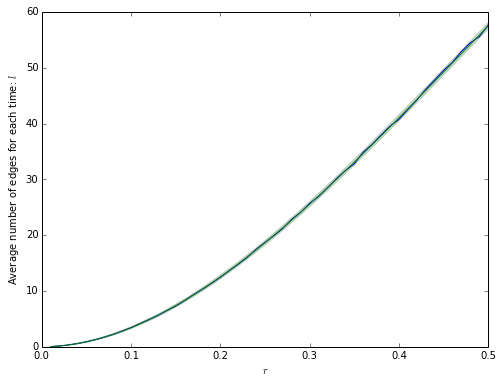
\includegraphics[width=10cm]{../img/r_l.png}
        \caption{$r$とクラスターの平均次数の関係}
        \label{fig:f23}
    \end{center}
\end{figure}
